\section{Introduction}

Cancer is a major public health problem worldwide and one of the leading death
causes. In 2012, there were an estimated 14.1 million new cancer cases with
estimated  8.2 million cancer deaths {\cite{cancer_stats_worldwide:2012}}. Lung
cancer is the most common cancer, both in terms of new cases (1.8 million) and
deaths (1.6 million). Breast  cancer is the second most common cancer (1.7
million cases) but only ranks 5th as cause of death (522,000 deaths). Colorectal
cancer (1.4 million cases; 694,000 deaths), prostate cancer (1.1 million cases;
307,000 deaths), stomach cancer (951,000 cases; 723,000 deaths) and liver cancer
(782,000 cases; 723,000 deaths) are following.

In Luxembourg, there were 1164 death cases caused by cancer in 2014, accounting
for 30.6\%  of the number of deaths. Cancer is thereby the second most common
death cause in Luxembourg, ranging behind cardiovascular diseases (1189 deaths;
31.3\%). Amongst these cancer deaths, cancers of the digestive organs (340
deaths) and of the respiratory organs (272 deaths) were the most frequent ones.
{\cite{cancer_stats:2012}}.

The accumulation of DNA mutations is a characteristic of tumors. Mutations in a
cell’s genetic material enable the so-called cancer hallmarks, which include,
amongst others, capabilities as activating invasion and metastasis, enabling
replicative immortality, sustaining proliferative signaling or evading growth
suppressors. Classical anti-cancer treatments are tailored for the \„average
patient\“ and not for the individual. Traditional cytotoxic chemotherapeutic
drugs, for instance, are unspecific and have numerous adverse effects [1]: they
attack rapidly dividing cells and make no difference between healthy and cancer
cells. For a long time, there was no possibility to predict the success of a
patient’s cancer treatment. In consequence, the treating clinician had no way to
personalize the treatment to the individual patient.

Personalized therapy by identification and targeting of tumor-specific molecular
abnormalities is rapidly becoming an important component in the management of
cancer patients. Consequently, algorithms for tumor diagnosis necessitate not
only morphological and immunophenotypic assessment of tumors but also molecular
mutational profiling. Among the solid tumors, mutational status is important to
the clinical management of patients with thyroid carcinomas, non-small cell
carcinomas of the lung, melanomas and colorectal carcinomas. In oncology, the
customized healthcare approach is designed to the individual patient by taking
into account the genetic information from a patient’s tumor biopsy. Targeting
proteins that give cancer cells a proliferative advantage, instead of simply
using cytotoxic agents, allows a more specific treatment and might decrease
treatment-associated side-effects. In the past years, the Food and Drug
Administration (FDA, USA) has approved several drugs that specifically target
proteins needed for cancerogenesis [2]. Many of these drugs are now effective
treatments for several common cancers. In many patients, however, these agents
might lack any efficiency: cancers are known to be highly heterogenous and
mutations in some subpopulations of cancer cells make them resistant to the
treatment [3]. Also, some of these targeted drugs can only be prescribed if the
targeted protein is not mutated, e.g. in wildtype status. Identifying these
mutations is thereby an utmost necessity for tailoring a targeted and efficient
cancer therapy. Amongst the many mutation detection techniques, Next Generation
Sequencing (NGS) constitutes the most powerful method and allows deep insights
into the underlying causes of diseases.

Critical alterations in cancer cells include single nucleotide variations (SNVs),
insertions and deletions of one or multiple nucleotides (INDELS), copy number
variations (CNVs) and rearrangements. Some of these variants are known to
provide increased sensitivity or resistance to targeted drugs. Whole-genome
(WGS) and whole-exome sequencing (WES) can detect these variants. These
experiments however are performed with low-coverage (100--250x in most
laboratories) and have thereby limited ability to detect somatic cancer variants
with the required confidence. In fact, cancers accumulate mutations and are
highly heterogeneous. A given small cancer subpopulation might present variants that
are absent to the rest of the cancer. This variant might be present at
low-frequency and might thereby not be detected in WGS or WES experiments. The
variant however might provide resistance to the treatment to cells in this
subpopulation. The cancer would eventually relapse. It is thereby of utmost
importance to gain deep insights into underlying genetic information to guide an
effective personalized therapy. This lead to the development of targeted NGS.

Next-Generation Sequencing (NGS) is a powerful method to analyze RNA or DNA
molecules. Improved protocols and methods have been developed in recent years
that allow to implement NGS for a variety of applications in both research and
diagnostics. NGS is still hard to implement and is mainly used in research. Only
a few laboratories are using this technique as a diagnostic technique.The SGMB
is building expertise in NGS and is implementing targeted NGS in its molecular
pathology laboratory. This implementation aims at gaining deep insights into the
underlying causes of solid tumors and in guiding targeted cancer therapy.

The completion of the human genome project and technical advances in the field
of genetics, in combination with advanced computer performance, enabled
geneticists and pharmacologists to adopt the personalization of cancer
diagnostics and treatment. The demand has driven the development of
high-throughput and faster sequencing: second-generation sequencing methods, or
NGS. NGS is also called massively parallel sequencing
as a massive amount of DNA fragments from a single sample are sequenced at the
same time. In the last decade, several benchtop sequencers have been developed
that provide high-throughput and cost-effective sequencing.

By identifying somatic mutations in cancer samples, NGS can guide personalized
cancer therapy approaches. The high-quality data produced by NGS can reveal
associations between several genes implicated in cancer subtypes and is thereby
of importance in drug development. In addition, it can be implemented in molecular
diagnostic laboratories to identify patients that would potentially benefit from
these targeted drugs.

Targeted NGS uses gene panels, e.g. only some regions in selected genes are
sequenced. The reduction of the regions of interest (ROIs) allows to significantly
increase the coverage. This allows a higher confidence and thereby enables
the implementation of NGS in diagnostic laboratories.

\subsection{EGFR Signaling in Cancer}

Bla {\cite{targeting_egfr:2012}}

Describe pathway

\begin{figure}[ht]
  \begin{center}
    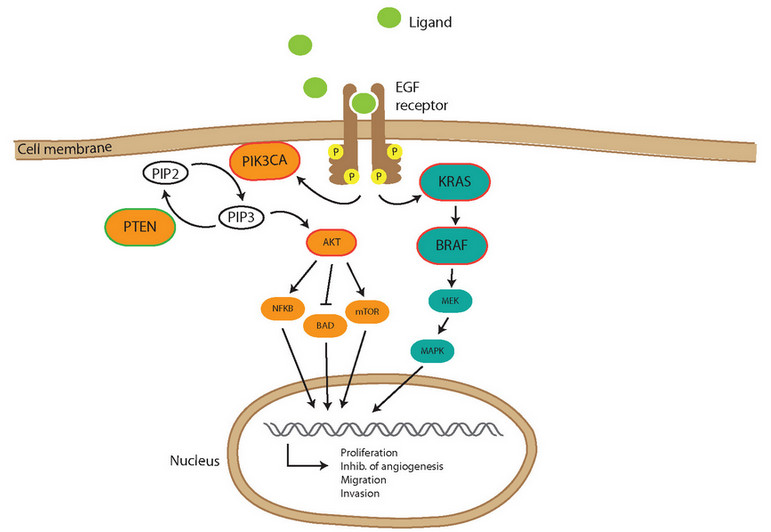
\includegraphics[scale=2,angle=0]{egfr_signaling.png}
    \caption{Schematic representation of the EGFR signaling cascade {\cite{targeting_egfr:2012}}}
    \label{Fig:egfr_signaling}
  \end{center}
\end{figure}

The samples analyzed in the SGMB originate from patients suffering from solid
tumors, mainly melanoma, non-small cell lung carcinoma (NSCLC), and colorectal
cancer. Evidence suggests that many solid tumors use and modify EGFR (Epithelial
Growth Factor Receptor) signaling for their purposes [4]. Targeting this
signaling pathway is thereby an attractive anti-cancer treatment. In this
regard, anti-EGFR monoclonal antibodies (cetuximab (Erbitux®) and panitumumab
(Vectibix®) and tyrosine kinase inhibitors (erlotinib (Tarceva®) and gefitinib
(Iressa®)) have shown their usefulness in cancer treatments [5]. EGFR and
downstream proteins K-Ras / N- Ras and B-Raf are predictive biomarkers for the
successfulness of the administration of the mentioned drugs [6]. Comprehensive
information about these markers is thereby essential when choosing a suitable
treatment in order to minimize treatment- associated side-effects and to
maximize the benefits of the treatment.

In their article, Scaltriti and Baselga present the EGFR signaling pathway as a
model for targeted therapy [7]. EGFR is part of the family of receptor tyrosine
kinases. This transmembrane protein is composed of an intracytoplasmic tyrosine
kinase domain, a short hydrophobic transmembrane region and an extracellular
ligand-binding domain. Upon ligand (EGF, TGFα) binding, EGFR becomes activated.
This leads to homodimerization, which results in an auto- and
cross-phosphorylation of key tyrosine residues on its cytoplasmic domain. This
forms docking sites for cytoplasmic proteins that contain
phosphotyrosine-binding and Src homology 2 domains. This allows, amongst others,
signaling through the PTEN/PI3K/AKT and RAS-RAF-MAPK pathways. Activation of
PTEN/PI3K/AKT leads to cell growth, proliferation and survival [8], while
RAS-RAF-MAPK induces cell survival and cell cycle progression and proliferation
[9]. In the RAS-Raf-MAPK pathway, Grb2 and Sos, two adaptor proteins, form a
complex with the activated EGFR [10]. The resulting conformational change of Sos
recruits Ras-GDP, which in turn becomes activated to form Ras-GTP. Ras-GTP
activates Raf, which, in intermediate steps, phosphorylates a MAPK
(mitogen-activated protein kinase). Activated MAPKs are then imported from the
cytoplasm into the nucleus where they act on target genes. The Ras and Raf
subfamilies include several proteins, three of them are of interest in targeted
cancer treatments: K-Ras, N-Ras and B-Raf.

In the past two decades, there has been increasing recognition that some somatic
mutations may be prognostic or predictive markers for specific therapies
available in colorectal cancer. These mutations involve genes such as KR​AS,
BRAF, PIK3CA, AKT1, SMAD4, PTEN, NRAS, and TGFBR2.

Lung cancer is comprised of two main histologic subtypes: non-small cell lung
cancer (NSCLC) and small cell lung cancer (SCLC). Over the past decade, it has
become evident that subsets of NSCLC can be further defined at the molecular
level by recurrent \'driver\' mutations that occur in multiple oncogenes,
including AKT1, ALK, BRAF, EGFR, HER2, KRAS, MEK1, MET, NRAS, PIK3CA, RET, and
ROS1 (Table 1). Another altered kinase gene involves MET. \'Driver\' mutations
lead to constitutive activation of mutant signaling proteins that induce and
sustain tumorigenesis. These mutations are rarely found concurrently in the same
tumor. Mutations can be found in all NSCLC histologies (including
adenocarcinoma, squamous cell carcinoma (SCC), and large cell carcinoma) and in
current, former, and never smokers (defined by individuals who smoked less than
100 cigarettes in a lifetime). Never smokers with adenocarcinoma have the
highest incidence of EGFR, HER2, ALK, RET, and ROS1 mutations. Importantly,
targeted small molecule inhibitors are currently available or being developed
for specific molecularly defined subsets of lung cancer patients.

Melanoma is a malignant tumor of melanocytes. The disease is the fifth most
common cancer in men and the seventh in women with an estimated 76,380 new cases
and 10,130 deaths in 2016 in the U.S. (ACS 2016). Melanoma is treated with a
combination of surgery, traditional cytotoxic chemotherapy, targeted therapies,
and immune-based therapies. Five-year survival rates for patients with
metastatic disease, unfortunately, are below 10\% (Jemal et al. 2010). Novel
therapies and treatment strategies are needed.

Historically, melanoma has been classified according to pathologic and clinical
characteristics such as histology (depth, Clark level, ulceration) and anatomic
site of origin. Over the past decade, it has become evident that subsets of
melanoma can be further defined at the molecular level by recurrent \"driver\"
mutations that occur in multiple oncogenes, including BRAF, GNA11, GNAQ, KIT,
MEK1 (MAP2K1), and NRAS (Table 1; Figure 1). Such driver mutations lead to
constitutive activation of mutant signaling proteins that induce and sustain
tumorigenesis.

Mutations in BRAF, GNA11, GNAQ, KIT, MEK1 (MAP2K1), and NRAS can be found in
approximately 70\% of all melanomas. In addition, mutations in CTNNB1 have also
been described in melanoma. Mutations in more than one of these genes are seldom
found concurrently in the same tumor. The distribution of mutations varies by
site of origin and also by the absence or presence of chronic sun damage (Table
1; Figure 1). Importantly, targeted small molecule inhibitors are currently
available or are being developed for specific molecular subsets of patients with
melanoma.

The Institut National du Cancer (F) [11]
provides recommendations about which mutations have to be searched to identify
patients eligible for the administration of monoclonal antibodies or tyrosine
kinase inhibitors. For instance, mutations on codon 12 and 13 in the KRAS gene
provide resistance to the monoclonal antibody agents panitumumab and cetuximab.
Gefinitinib, a tyrosine kinase inhibitor, can only be prescribed for patients,
which show no activating mutations on EGFR.


EGFR-targeted drugs:
bevacizumab, cetuximab, panitumumab, ...

\subsection{Targeted Sequencing and Target Enrichment Methods}

Targeted sequencing to a depth that allows detection of relatively low mutant
allele frequency (MAF) may represent an alternative or a complement to WGS and
WES to detect clinically relevant alterations. Additionally, in most clinical
and research settings, the amount of DNA that can be isolated from tumor samples
is limited and the DNA is often damaged owing to fixation and storage procedures
such as those used with formalin-fixed paraffin-embedded (FFPE) samples.
Therefore a multiplexed targeted platform that can generate reliable data with
high sensitivity from limited amounts of DNA from FFPE samples is needed.
Several targeted sequencing panels have been successfully implemented (6, 7).
However, the details of a platform's design and parameterization will influence
the precision and reliability of the molecular profiling results, impacting both
translational research and clinical decision-making. Thus, it is of great value
to explore multiple potential solutions in a real patient care environment until
a community-wide solution is established, validated, and well accepted.

Benchtop sequencing devices: more labs can now do sequencing as it becomes
faster \& cheaper \& more reliable.Several NGS bench-top devices have become
available in the last decade. These instrumentations differ in their underlying
chemistry that influences the instrument’s performance, accuracy, output and
time per run. Common sequencing principles include pyrosequencing (454),
sequencing by ligation (SOLiD), ion semiconductor (Ion Torrent) and sequencing
by synthesis (Illumina) [12]. Even though advances in sequencing technology and
computational power and tools have decreased the time and cost of a sequencing
experiment, NGS is still mainly used in research, with only a few laboratories
using this technique in diagnostics.

In fact, validation of a NGS methodology requires careful assessment of methods
and tools [13]. Therefore, each step that is performed from the initial starting
material to sample processing, sequencing library preparation, sequencing assay
and bioinformatic processing has to be carefully checked for sources of
potential errors or variability. Basically, in the validation process, it is
checked whether the method measures what it claims to measure with the required
sensitivity and sensibility.

With the success of NGS, many cancer genomes have been sequenced and made
available to the worldwide research community. Companies, molecular diagnostics
laboratories and academic centers are trying to use these big data for their
purposes. A lot of mutations are described in these genomes, but only a small
fraction of them are clinically actionable, e.g. can be targeted with specific
drugs. Therefore, a molecular pathology laboratory does not need to perform
whole-genome or -exome sequencing, but can employ targeted NGS to analyze some
genes of interest, which include mutations for which there exists a clinical
utility. Due to the low number of target regions, targeted NGS allows high
coverage. In addition, it is a time- and cost- efficient alternative to
whole-genome or -exome sequencing. Also, targeted NGS results in a significantly
lower amount of produced data and thereby eases data storage and analysis time.
Table 1 shows a selection of commercially available cancer gene panels, which
all allow to analyze selected regions of genes implicated in cancerogenesis.
Before implementing one of these panels for molecular diagnostics, it has to be
ensured that the panel allows to study the genes of interest, e.g. genes that
are clinically applicable, and a careful assessment of its analytical validity
has to be performed.

More \& more databases describing SNPs \& known pathogenic hotspots

Bla {\cite{enrichment_methods:2011}}

Hybrid capture

Selective circularization

PCR amplification

\subsection{Sequencing Chemistries}

IonTorrent, etc

\subsubsection{Illumina MiSeq}

http://www.illumina.com/documents/products/techspotlights/techspotlight_sequencing.pdf

Illumina sequencing technology leverages clonal array formation and proprietary reversible terminator technology for rapid and accurate large-scale sequencing. The innovative and  exible sequencing system enables a broad array of applications in genomics, transcriptomics, and epigenomics.

Sequencing templates are immobilized on a proprietary  ow cell surface (Figure 1) designed to present the DNA in a manner that facilitates access to enzymes while ensuring high stability of surface- bound template and low non-speci c binding of  uorescently labeled nucleotides. Solid-phase ampli cation (Figures 2–7) creates up to 1,000 identical copies of each single template molecule in close prox- imity (diameter of one micron or less). Because this process does not involve photolithography, mechanical spotting, or positioning of beads into wells, densities on the order of ten million single-molecule clusters per square centimeter are achieved.

The Illumina sequencing approach is built around a massive quantity of sequence reads in parallel. Deep sampling and uniform coverage is used to generate a consensus and ensure high con dence in determination of genetic differences. Deep sampling allows the use of weighted majority voting and statistical analysis, similar to conventional methods, to identify homozygotes and heterozygotes and to distin- guish sequencing errors. Each raw read base has an assigned quality score so that the software can apply a weighting factor in calling differ- ences and generating con dence scores.

Illumina data collection software enables users to align sequences to a reference in resequencing applications (Figure 13). Developed in collaboration with leading researchers, this software suite includes the full range of data collection, processing, and analysis modules to streamline collection and analysis of data with minimal user interven- tion. The open format of the software allows easy access to data at various stages of processing and analysis using simple application program interfaces.

https://en.wikipedia.org/wiki/Illumina_dye_sequencing

Illumina dye sequencing is a technique used to determine the series of base pairs in DNA, also known as DNA sequencing. The reversible terminated chemistry concept was invented by Bruno Canard and Simon Sarfati at the Pasteur Institute in Paris.[1][2] It was developed by Shankar Balasubramanian and David Klenerman of Cambridge University,[3] who subsequently founded Solexa, a company later acquired by Illumina. This sequencing method is based on reversible dye-terminators that enable the identification of single bases as they are introduced into DNA strands. It can also be used for whole-genome and region sequencing, transcriptome analysis, metagenomics, small RNA discovery, methylation profiling, and genome-wide protein-nucleic acid interaction analysis.[4][5]

(amfong net :) The first step after DNA purification is tagmentation. Enzymes called transposomes randomly cut the DNA into short segments (“tags”). Adapters are added on either side of the cut points (ligation). Strands that fail to have adapters ligated are washed away.[6])

The next step is called reduced cycle amplification. During this step, sequences for primer binding, indices, and terminal sequences are added. Indices are usually six base pairs long and are used during DNA sequence analysis to identify samples. Indices allow for up to 96 different samples to be run together. During analysis, the computer will group all reads with the same index together.[7][8] The terminal sequences are used for attaching the DNA strand to the flow cell. Illumina uses a “sequence by synthesis” approach.[8] This process takes place inside of an acrylamide-coated glass flow cell.[9] The flow cell has oligonucleotides (short nucleotide sequences) coating the bottom of the cell, and they serve to hold the DNA strands in place during sequencing. The oligos match the two kinds of terminal sequences added to the DNA during reduced cycle amplification. As the DNA enters the flow cell, one of the adapters attaches to a complementary oligo.

Once attached, cluster generation can begin. The goal is to create hundreds of identical strands of DNA. Some will be the forward strand; the rest, the reverse. Clusters are generated through bridge amplification. Polymerases move along a strand of DNA, creating its complementary strand. The original strand is washed away, leaving only the reverse strand. At the top of the reverse strand there is an adapter sequence. The DNA strand bends and attaches to the oligo that is complementary to the top adapter sequence. Polymerases attach to the reverse strand, and its complementary strand (which is identical to the original) is made. The now double stranded DNA is denatured so that each strand can separately attach to an oligonucleotide sequence anchored to the flow cell. One will be the reverse strand; the other, the forward. This process is called bridge amplification, and it happens for thousands of clusters all over the flow cell at once.

Over and over again, DNA strands will bend and attach to oligos. Polymerases will synthesize a new strand to create a double stranded segment, and that will be denatured so that all of the DNA strands in one area are from a single source (clonal amplification). Clonal amplification is important for quality control purposes. If a strand is found to have an odd sequence, then scientists can check the reverse strand to make sure that it has the complement of the same oddity. The forward and reverse strands act as checks to guard against artifacts. Because Illumina sequencing uses polymerases, base substitution errors have been observed,[10] especially at the 3’ end.[11] Paired end reads combined with cluster generation can confirm an error took place. The reverse and forward strands should be complementary to each other, all reverse reads should match each other, and all forward reads should match each other. If a read is not similar enough to its counterparts (with which it should be a clone), an error may have occurred. A minimum threshold of 97% similarity has been used in some labs’ analyses.[11]

At the end of bridge amplification, all of the reverse strands are washed off the flow cell, leaving only forward strands. Primers attach to the forward strands and add fluorescently tagged nucleotides to the DNA strand. Only one base is added per round. A reversible terminator is on every nucleotide to prevent multiple additions in one round. Each of the four bases has a unique emission, and after each round, the machine records which base was added. This process is “sequence by synthesis.”

Once the DNA strand has been read, the strand that was just added is washed away. Then, the index 1 primer attaches, polymerizes the index 1 sequence, and is washed away. The strand forms a bridge again, and the 3’ end of the DNA strand attaches to an oligo on the flow cell. The index 2 primer attaches, polymerizes the sequence, and is washed away.

A polymerase sequences the complementary strand on top of the arched strand. They separate, and the 3’ end of each strand is blocked. The forward strand is washed away, and the process of sequence by synthesis repeats for the reverse strand.

The sequencing occurs for millions of clusters at once, and each cluster has ~1,000 identical copies of a DNA insert.[10] The sequence data is analyzed by finding fragments with overlapping areas, called contigs, and lining them up. If a reference sequence is known, the contigs are then compared to it for variant identification.

This piecemeal process allows scientists to see the complete sequence even though an unfragmented sequence was never run; however, because Illumina read lengths are not very long [11] (HiSeq sequencing can produce read lengths around 90 bp long [7]), it can be a struggle to resolve short tandem repeat areas.[7][10] Also, if the sequence is de novo and so a reference doesn’t exist, repeated areas can cause a lot of difficulty in sequence assembly.[10] Additional difficulties include base substitutions (especially at the 3’ end of reads[11]) by inaccurate polymerases, chimeric sequences, and PCR-bias, all of which can contribute to generating an incorrect sequence.[11]



\subsection{NGS Data Analysis}

GATK best practices

\subsection{Practical Implications in the Laboratory}

Chemical fixatives are used to preserve tissue from degradation, and to maintain
the structure of the cell and of sub-cellular components such as cell organelles
(e.g., nucleus, endoplasmic reticulum, mitochondria). The most common fixative
for light microscopy is 10\% neutral buffered formalin (4\% formaldehyde in
phosphate buffered saline).

These fixatives preserve tissues or cells mainly by irreversibly cross-linking
proteins. The main action of these aldehyde fixatives is to cross-link amino
groups in proteins through the formation of methylene bridges (-CH2-), in the
case of formaldehyde.

This process, while preserving the structural integrity of the cells and tissue
can damage the biological functionality of proteins, particularly enzymes, and
can also denature them to a certain extent. This can be detrimental to certain
histological techniques.

Formalin fixation leads to degradation of mRNA, miRNA and DNA in tissues.
However, extraction, amplification and analysis of these nucleic acids from
formalin-fixed, paraffin-embedded tissues is possible using appropriate
protocols.

The aim of Tissue Processing is to remove water from tissues and replace with a
medium that solidifies to allow thin sections to be cut. Biological tissue must
be supported in a hard matrix to allow sufficiently thin sections to be cut,
typically 5 μm (micrometres; 1000 micrometres = 1 mm) thick for light microscopy.

Since it is immiscible with water, the main constituent of biological tissue,
water must first be removed in the process of dehydration. Samples are
transferred through baths of progressively more concentrated ethanol to remove
the water. This is followed by a hydrophobic clearing agent (such as xylene) to
remove the alcohol, and finally molten paraffin wax, the infiltration agent,
which replaces the xylene. Paraffin wax does not provide a sufficiently hard
matrix for cutting very thin sections for electron microscopy. Instead, resins
are used. Epoxy resins are the most commonly employed embedding media, but
acrylic resins are also used, particularly where immunohistochemistry is
required. Thicker sections (0.35μm to 5μm) of resin-embedded tissue can also be
cut for light microscopy. Again, the immiscibility of most epoxy and acrylic
resins with water necessitates the use of dehydration, usually with ethanol.

After the tissues have been dehydrated, cleared, and infiltrated with the
embedding material, they are ready for external embedding. During this process
the tissue samples are placed into molds along with liquid embedding material
(such as agar, gelatine, or wax) which is then hardened. This is achieved by
cooling in the case of paraffin wax and heating (curing) in the case of the
epoxy resins. The acrylic resins are polymerised by heat, ultraviolet light, or
chemical catalysts. The hardened blocks containing the tissue samples are then
ready to be sectioned.

Because Formalin-fixed, paraffin-embedded (FFPE) tissues may be stored
indefinitely at room temperature, and nucleic acids (both DNA and RNA) may be
recovered from them decades after fixation, FFPE tissues are an important
resource for historical studies in medicine.

For light microscopy, a steel knife mounted in a microtome is used to cut
4-micrometer-thick tissue sections which are mounted on a glass microscope
slide. For transmission electron microscopy, a diamond knife mounted in an
ultramicrotome is used to cut 50-nanometer-thick tissue sections which are
mounted on a 3-millimeter-diameter copper grid. Then the mounted sections are
treated with the appropriate stain.

The quality of the genetic testing of the tumor is affected by several factors.
These include the content of tumor cells in the sample, the quality of the
tissue material, sequencing library preparation and the the bioinformatic
pipeline.

The biopsy usually consists of an admixture of normal and cancer cells. The
sensitivity of tumor variant detection is linked to the tumor cell content of
the specimen. In addition, cancers are highly heterogenous, e.g. a small
subpopulation might present mutations that provide resistance to targeted
treatment. Detecting these low-frequency mutations and clearly separating them
from eventual high-frequency fixation or sequencing artifacts presents a huge
challenge [14].

Tumor biopsies usually yield a limited amount of tissue, therefore it is
conceivable to use the same sample for more analyses. In Luxembourg, all
relevant tumor biopsies are usually sent to the Laboratoire National de Santé
(LNS) to the Service of Pathologic Anatomy where the biopsy is fixed in formalin
and embedded in paraffin (FFPE). FFPE conserves the tissue morphology and
thereby allows histological analysis. In addition, it allows to store specimens
for decades. Sample quality, however, is influenced by this fixation method, but
also by the size of the biopsy, and its fixation time [13]. DNA extraction from
FFPE samples is difficult and yields low amounts of DNA [15]; formaldehyde leads
to cross-linking of nucleic acids and proteins [16]; FFPE introduces fixation
artifacts into DNA sequences [17|. These circumstances complicate sample
processing as well as NGS data interpretation. Though, FFPE samples have been
shown to be still suitable for downstream analyses [18].

Sequencing library preparation also affects the final NGS result. Several
technologies for target enrichment exist and are available for different
sequencing instruments [19]. Essential for all these enrichment methods is the
amplification of target regions and the introduction of multiplexing, which
requires the incorporation of a unique index adaptor combination for each
sample. Target enrichment methods can be separated into three basic groups:
targeted circularization, hybrid capture of target fragments and PCR-based
enrichment methods. PCR-driven methods happen on high-molecular DNA. In contrast
to uniplex long-range PCR, short-range multiplex PCR produces short DNA
fragments of target regions. There is thereby no need of DNA shearing.
Hybridization-based methods require a so-called shotgun library construction
before target regions can be captured. During this process, genomic DNA is
sheared randomly into small fragments and an adapter- and index-linked library
is produced. Biotinylated baits are added that bind to target regions. Target
regions can then be captured using streptadivin coated magnetic beads. Targeted
circularization methods rely on a digestion of DNA by restriction enzymes. The
produced DNA fragments are then circularized and uncircularized DNA fragments
are removed by exonucleases. Only circularized target regions are then amplified
by PCR.

The establishment and validation of a bioinformatic NGS data analysis pipeline
still constitutes a challenge in diagnostics. After generation of FASTQ files of
the sequencer, data generally undergo quality control, followed by trimming of
low quality bases, alignment to the reference genome, variant calling and
variant annotation. For each of these steps, several bioinformatic algorithms
and tools exist [20]. The computational pipeline of the molecular pathology
laboratory has to incorporate the tools that allow the most sensitive and
sensible analysis of data. For instance, quality trimming influences the mapping
to the reference genome. The mapping, in turn, strongly affects the variant
calling. In fact, variant calling is a critical step in NGS data analysis.
Several tool kits as SAMtools, SPLINTER, VarScan2 or GATK allow variant
annotation, but vary in their false-positive and false-negative detection rates
([21], [22]). These tools have to be carefully assessed, as false-positives or
false-negatives should absolutely be avoided when it comes to the subscription
of a targeted chemotherapeutic agent.

To facilitate interpretation of NGS data, variants have to be annotated and their clinical actionability has to be identified. Several databases have emerged in this field (such as mycancergenome.org) and numerous tools allow to automatize variant annotation. Here again, the choice of the database and the variant annotator is important.

Finally, the sample-to-results time is a very pragmatic, but important factor. The time from the biopsy to the potential start of an administration of a targeted chemotherapeutic drug should be reduced to a minimum. For instance, in case of late-stage cancer patients, it would be unacceptable if analysis would take several weeks. To reduce the sample-to-results time to under two weeks, the sample processing workflow should be as short as possible, while still yielding high quality sequencing libraries. The bioinformatic pipeline should not only incorporate the best tools, but should also be automatized to further reduce the time of analysis.
=======
Chemical fixatives are used to preserve tissue from degradation, and to maintain
the structure of the cell and of sub-cellular components such as cell organelles
(e.g., nucleus, endoplasmic reticulum, mitochondria). The most common fixative
for light microscopy is 10% neutral buffered formalin (4% formaldehyde in
phosphate buffered saline).

These fixatives preserve tissues or cells mainly by irreversibly cross-linking
proteins. The main action of these aldehyde fixatives is to cross-link amino
groups in proteins through the formation of methylene bridges (-CH2-), in the
case of formaldehyde.

This process, while preserving the structural integrity of the cells and tissue
can damage the biological functionality of proteins, particularly enzymes, and
can also denature them to a certain extent. This can be detrimental to certain
histological techniques.

Formalin fixation leads to degradation of mRNA, miRNA and DNA in tissues.
However, extraction, amplification and analysis of these nucleic acids from
formalin-fixed, paraffin-embedded tissues is possible using appropriate
protocols.

The aim of Tissue Processing is to remove water from tissues and replace with a
medium that solidifies to allow thin sections to be cut. Biological tissue must
be supported in a hard matrix to allow sufficiently thin sections to be cut,
typically 5 μm (micrometres; 1000 micrometres = 1 mm) thick for light microscopy.

Since it is immiscible with water, the main constituent of biological tissue,
water must first be removed in the process of dehydration. Samples are
transferred through baths of progressively more concentrated ethanol to remove
the water. This is followed by a hydrophobic clearing agent (such as xylene) to
remove the alcohol, and finally molten paraffin wax, the infiltration agent,
which replaces the xylene. Paraffin wax does not provide a sufficiently hard
matrix for cutting very thin sections for electron microscopy. Instead, resins
are used. Epoxy resins are the most commonly employed embedding media, but
acrylic resins are also used, particularly where immunohistochemistry is
required. Thicker sections (0.35μm to 5μm) of resin-embedded tissue can also be
cut for light microscopy. Again, the immiscibility of most epoxy and acrylic
resins with water necessitates the use of dehydration, usually with ethanol.

After the tissues have been dehydrated, cleared, and infiltrated with the
embedding material, they are ready for external embedding. During this process
the tissue samples are placed into molds along with liquid embedding material
(such as agar, gelatine, or wax) which is then hardened. This is achieved by
cooling in the case of paraffin wax and heating (curing) in the case of the
epoxy resins. The acrylic resins are polymerised by heat, ultraviolet light, or
chemical catalysts. The hardened blocks containing the tissue samples are then
ready to be sectioned.

Because Formalin-fixed, paraffin-embedded (FFPE) tissues may be stored
indefinitely at room temperature, and nucleic acids (both DNA and RNA) may be
recovered from them decades after fixation, FFPE tissues are an important
resource for historical studies in medicine.

For light microscopy, a steel knife mounted in a microtome is used to cut
4-micrometer-thick tissue sections which are mounted on a glass microscope
slide. For transmission electron microscopy, a diamond knife mounted in an
ultramicrotome is used to cut 50-nanometer-thick tissue sections which are
mounted on a 3-millimeter-diameter copper grid. Then the mounted sections are
treated with the appropriate stain.

quantitation

ffpe quality control necessary. FFPE are degraded. More C>T

Target enrichment methods hun och vlt en effekt

choice vum sequencer, different error rates, different yield, analysis time.

choice vun den bioinformatic tools. t'gin der vill, vir- an nodeeler. zB variant
calling algorithms: most are for haplotypes and not for somatic variants. many
need matched tumor-normal samples, which we here in the lab do not have, only have
tumor dna. after variant calling, they have to be annotated for their clinical
relevance and potential actionability.

problem: many variants may be found, some of them may be
harmless germline SNPs, many variants may be causative of cancer, but are not actionable.

time sample-to-result

how to report? all results or only those that are known to be actionable.
>>>>>>> a5147a619d3523c598b91a86e2c62e19a96fd26f

\subsection{Aims of the Thesis}
Targeted NGS is still not widely used in diagnostics laboratories. The SGMB of the LNS
is planning to build expertise with the aim to adopt NGS routinely in the laboratory,
mainly in the context of diagnosis and therapy of cancer patients in Luxembourg.

The aim of this thesis project was to test commercially available cancer gene panels,
e.g. Illumina Trusight Tumor 15 and Agilent Haloplex HS ClearSeq Cancer, for their
potential use in the routine workflow of the laboratory. Several samples of cancer
patients were prepared with both kits and were sequenced on the Illumina MiSeq device.
Both kits vary in their sequencing library preparation principles: Illumina's tst15
uses the multiplex PCR approach while Agilent's Haloplex Enrichment System uses
enzymatic DNA restriction followed by probe capture.

NGS data were analyzed with the respective recommended pipelines and a custom in-house
pipeline.

Finally, several freely available variant calling algorithms were tested for their
potential implementation in the custom in-house variant discovery bioinformatic
pipeline.
